% Options for packages loaded elsewhere
\PassOptionsToPackage{unicode}{hyperref}
\PassOptionsToPackage{hyphens}{url}
%
\documentclass[
]{article}
\usepackage{amsmath,amssymb}
\usepackage{lmodern}
\usepackage{ifxetex,ifluatex}
\ifnum 0\ifxetex 1\fi\ifluatex 1\fi=0 % if pdftex
  \usepackage[T1]{fontenc}
  \usepackage[utf8]{inputenc}
  \usepackage{textcomp} % provide euro and other symbols
\else % if luatex or xetex
  \usepackage{unicode-math}
  \defaultfontfeatures{Scale=MatchLowercase}
  \defaultfontfeatures[\rmfamily]{Ligatures=TeX,Scale=1}
\fi
% Use upquote if available, for straight quotes in verbatim environments
\IfFileExists{upquote.sty}{\usepackage{upquote}}{}
\IfFileExists{microtype.sty}{% use microtype if available
  \usepackage[]{microtype}
  \UseMicrotypeSet[protrusion]{basicmath} % disable protrusion for tt fonts
}{}
\makeatletter
\@ifundefined{KOMAClassName}{% if non-KOMA class
  \IfFileExists{parskip.sty}{%
    \usepackage{parskip}
  }{% else
    \setlength{\parindent}{0pt}
    \setlength{\parskip}{6pt plus 2pt minus 1pt}}
}{% if KOMA class
  \KOMAoptions{parskip=half}}
\makeatother
\usepackage{xcolor}
\IfFileExists{xurl.sty}{\usepackage{xurl}}{} % add URL line breaks if available
\IfFileExists{bookmark.sty}{\usepackage{bookmark}}{\usepackage{hyperref}}
\hypersetup{
  pdftitle={ipmr\_analysis},
  pdfauthor={Alice Stears},
  hidelinks,
  pdfcreator={LaTeX via pandoc}}
\urlstyle{same} % disable monospaced font for URLs
\usepackage[margin=1in]{geometry}
\usepackage{color}
\usepackage{fancyvrb}
\newcommand{\VerbBar}{|}
\newcommand{\VERB}{\Verb[commandchars=\\\{\}]}
\DefineVerbatimEnvironment{Highlighting}{Verbatim}{commandchars=\\\{\}}
% Add ',fontsize=\small' for more characters per line
\usepackage{framed}
\definecolor{shadecolor}{RGB}{248,248,248}
\newenvironment{Shaded}{\begin{snugshade}}{\end{snugshade}}
\newcommand{\AlertTok}[1]{\textcolor[rgb]{0.94,0.16,0.16}{#1}}
\newcommand{\AnnotationTok}[1]{\textcolor[rgb]{0.56,0.35,0.01}{\textbf{\textit{#1}}}}
\newcommand{\AttributeTok}[1]{\textcolor[rgb]{0.77,0.63,0.00}{#1}}
\newcommand{\BaseNTok}[1]{\textcolor[rgb]{0.00,0.00,0.81}{#1}}
\newcommand{\BuiltInTok}[1]{#1}
\newcommand{\CharTok}[1]{\textcolor[rgb]{0.31,0.60,0.02}{#1}}
\newcommand{\CommentTok}[1]{\textcolor[rgb]{0.56,0.35,0.01}{\textit{#1}}}
\newcommand{\CommentVarTok}[1]{\textcolor[rgb]{0.56,0.35,0.01}{\textbf{\textit{#1}}}}
\newcommand{\ConstantTok}[1]{\textcolor[rgb]{0.00,0.00,0.00}{#1}}
\newcommand{\ControlFlowTok}[1]{\textcolor[rgb]{0.13,0.29,0.53}{\textbf{#1}}}
\newcommand{\DataTypeTok}[1]{\textcolor[rgb]{0.13,0.29,0.53}{#1}}
\newcommand{\DecValTok}[1]{\textcolor[rgb]{0.00,0.00,0.81}{#1}}
\newcommand{\DocumentationTok}[1]{\textcolor[rgb]{0.56,0.35,0.01}{\textbf{\textit{#1}}}}
\newcommand{\ErrorTok}[1]{\textcolor[rgb]{0.64,0.00,0.00}{\textbf{#1}}}
\newcommand{\ExtensionTok}[1]{#1}
\newcommand{\FloatTok}[1]{\textcolor[rgb]{0.00,0.00,0.81}{#1}}
\newcommand{\FunctionTok}[1]{\textcolor[rgb]{0.00,0.00,0.00}{#1}}
\newcommand{\ImportTok}[1]{#1}
\newcommand{\InformationTok}[1]{\textcolor[rgb]{0.56,0.35,0.01}{\textbf{\textit{#1}}}}
\newcommand{\KeywordTok}[1]{\textcolor[rgb]{0.13,0.29,0.53}{\textbf{#1}}}
\newcommand{\NormalTok}[1]{#1}
\newcommand{\OperatorTok}[1]{\textcolor[rgb]{0.81,0.36,0.00}{\textbf{#1}}}
\newcommand{\OtherTok}[1]{\textcolor[rgb]{0.56,0.35,0.01}{#1}}
\newcommand{\PreprocessorTok}[1]{\textcolor[rgb]{0.56,0.35,0.01}{\textit{#1}}}
\newcommand{\RegionMarkerTok}[1]{#1}
\newcommand{\SpecialCharTok}[1]{\textcolor[rgb]{0.00,0.00,0.00}{#1}}
\newcommand{\SpecialStringTok}[1]{\textcolor[rgb]{0.31,0.60,0.02}{#1}}
\newcommand{\StringTok}[1]{\textcolor[rgb]{0.31,0.60,0.02}{#1}}
\newcommand{\VariableTok}[1]{\textcolor[rgb]{0.00,0.00,0.00}{#1}}
\newcommand{\VerbatimStringTok}[1]{\textcolor[rgb]{0.31,0.60,0.02}{#1}}
\newcommand{\WarningTok}[1]{\textcolor[rgb]{0.56,0.35,0.01}{\textbf{\textit{#1}}}}
\usepackage{graphicx}
\makeatletter
\def\maxwidth{\ifdim\Gin@nat@width>\linewidth\linewidth\else\Gin@nat@width\fi}
\def\maxheight{\ifdim\Gin@nat@height>\textheight\textheight\else\Gin@nat@height\fi}
\makeatother
% Scale images if necessary, so that they will not overflow the page
% margins by default, and it is still possible to overwrite the defaults
% using explicit options in \includegraphics[width, height, ...]{}
\setkeys{Gin}{width=\maxwidth,height=\maxheight,keepaspectratio}
% Set default figure placement to htbp
\makeatletter
\def\fps@figure{htbp}
\makeatother
\setlength{\emergencystretch}{3em} % prevent overfull lines
\providecommand{\tightlist}{%
  \setlength{\itemsep}{0pt}\setlength{\parskip}{0pt}}
\setcounter{secnumdepth}{-\maxdimen} % remove section numbering
\ifluatex
  \usepackage{selnolig}  % disable illegal ligatures
\fi

\title{ipmr\_analysis}
\author{Alice Stears}
\date{12/10/2021}

\begin{document}
\maketitle

\hypertarget{background}{%
\section{Background}\label{background}}

\emph{Oenothera coloradensis} is a monocarpic perennial herb that occurs
riparian adn wetland habitats in southeast Wyoming, southwest Nebraska,
and northern Colorado. It was listed as ``threatened'' under the
Endangered Species Act until December, 2019. It was orginially listed
because it is naturally rare, and even though it's ESA designation has
since been removed, this species is still very uncommon. One chapter of
my dissertation is using demographic methods to investigate the
mechansisms that allow populations of this rare species to persist. I am
building an integral projection model (IPM) for this species, and can
use results from this model to test several persistence mechanisms.

I have three consecutive years of pre-reproductive census data for this
species, which includes survival status, size (longest leaf),
reproductive status, and reproductive output for each year. I also have
counts of `seedlings' in each year (individuals less than 3 cm in leaf
length), and estimates of seed germination rate and seed vitality rate.
I am working on building an IPM that includes a continuous stage for
adult individuals, and two discrete stages for seedlings and the
seedbank. I was able to build a test IPM using only the continuous stage
by hand using code from Ellner and Rees, 2016. However, the process for
creating an IPM by hand with two discrete stages as well as a continuous
stage seemed daunting, so I've tried to use the \texttt{ipmr} package.
I've followed the \texttt{ipmr} vignettes and was able to create a
simple, continuos-only IPM in impr that returns the same results as the
continous-only IPM I built by hand. However, because the package is new
and there is not a published example of an ipm with two discrete stages,
I'm not as confident as I'd like that I've specified the general,
multi-stage model correctly. I would greatly appreciate you taking a
quick look at the model, and if possible confirming that I've specified
it correctly. I've included a life-cycle diagram for this species, the
IPM kernel functions, and code for a general, discrete ipm with one
continous and two discrete stages I've created using \texttt{ipmr}. This
model doesn't include density dependence and environmental co-variates,
since I've been able to follow the \texttt{ipmr} vignettes to
incorporate these elements. I'm primarily interested in confirming that
I've written the code for the demographic functions correctly.

\hypertarget{oenothera-coloradensis-life-cycle-diagram}{%
\subsubsection{\texorpdfstring{\emph{Oenothera coloradensis} life-cycle
diagram}{Oenothera coloradensis life-cycle diagram}}\label{oenothera-coloradensis-life-cycle-diagram}}

Here is a diagram of the life-cyle of \emph{Oenothera coloradensis}. All
of the transitions included in the IPM are labeled.
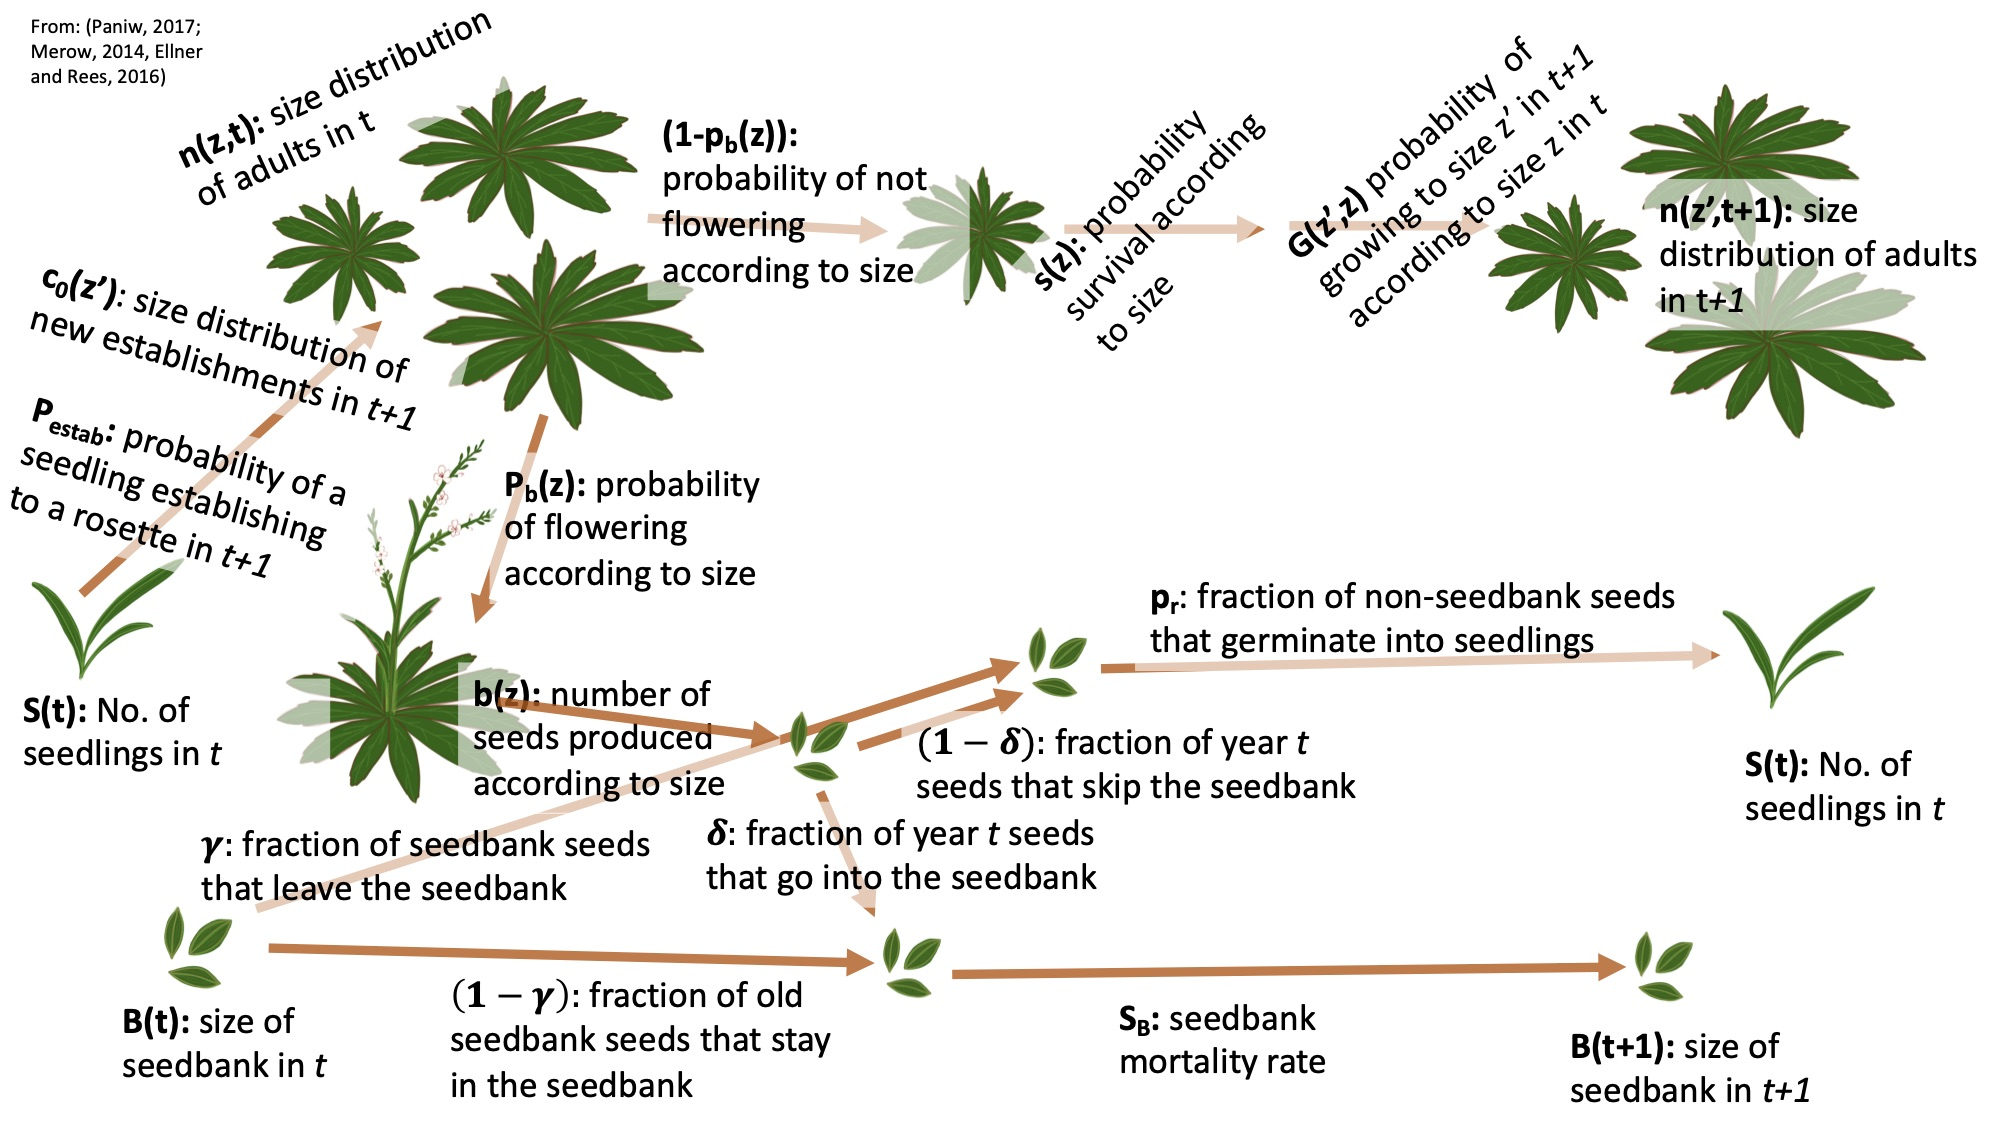
\includegraphics{/Users/Alice/Dropbox/Grad School/Research/Oenothera coloradensis project/COBP_analysis/images/COBP_lifecyclediagram.jpg}

\hypertarget{functions-in-the-ipm-kernel}{%
\subsubsection{Functions in the IPM
kernel}\label{functions-in-the-ipm-kernel}}

\textbf{Distribution of size of individuals in year \emph{t+1}
(continuous stage):} New recruits from the seedling stage + growth and
survival kernel
\[n(z',t+1) = S(t)p_{estab}c_o(z') + \int_{L}^{U}(1-P_b(z))s(z)G(z',z)n(z,t)dz \]
\textbf{Size of the seedling stage (discrete stage):}
\[S(t+1) = B(t)outSB + goSdlng\int_{L}^{U}P_b(z)b(z)n(z,t)dz \]

\textbf{Seedbank (discrete stage):} (after Ellner, 2016)
\[B(t+1) = B(t)staySB+goSB\int_{L}^{U}P_b(z)b(z)n(z,t)dz \]

\hypertarget{load-oenothera-coloradensis-census-data}{%
\section{\texorpdfstring{Load \emph{Oenothera coloradensis} census
data}{Load Oenothera coloradensis census data}}\label{load-oenothera-coloradensis-census-data}}

\begin{Shaded}
\begin{Highlighting}[]
\CommentTok{\# load continuous stage data}
\NormalTok{dat }\OtherTok{\textless{}{-}} \FunctionTok{read.csv}\NormalTok{(}\StringTok{"../../Processed\_Data/COBP\_long\_CURRENT.csv"}\NormalTok{)}
\NormalTok{discreteDat }\OtherTok{\textless{}{-}} \FunctionTok{read.csv}\NormalTok{(}\StringTok{"../../Processed\_Data/discreteStageData.csv"}\NormalTok{)}
\end{Highlighting}
\end{Shaded}

\hypertarget{make-vital-rate-models}{%
\section{Make vital rate models}\label{make-vital-rate-models}}

These are simple models that do not include density dependence or
environmental covariates, although the final models will contain these
elements. \#\#\# Survival (\(s(z)\))

\begin{Shaded}
\begin{Highlighting}[]
\DocumentationTok{\#\# subset the data to exclude flowering individuals}
\NormalTok{survDat }\OtherTok{\textless{}{-}}\NormalTok{ dat[dat}\SpecialCharTok{$}\NormalTok{flowering}\SpecialCharTok{==}\DecValTok{0} \SpecialCharTok{|} \FunctionTok{is.na}\NormalTok{(dat}\SpecialCharTok{$}\NormalTok{flowering),]}

\DocumentationTok{\#\# logistic glm with log{-}transformed size\_t}
\NormalTok{survMod }\OtherTok{\textless{}{-}} \FunctionTok{glm}\NormalTok{(survives\_tplus1 }\SpecialCharTok{\textasciitilde{}}\NormalTok{ log\_LL\_t , }\AttributeTok{data =}\NormalTok{ survDat, }\AttributeTok{family =}\NormalTok{ binomial)}
\FunctionTok{summary}\NormalTok{(survMod)}
\end{Highlighting}
\end{Shaded}

\begin{verbatim}
## 
## Call:
## glm(formula = survives_tplus1 ~ log_LL_t, family = binomial, 
##     data = survDat)
## 
## Deviance Residuals: 
##     Min       1Q   Median       3Q      Max  
## -1.8139  -1.3476   0.8149   0.9412   1.2158  
## 
## Coefficients:
##             Estimate Std. Error z value Pr(>|z|)    
## (Intercept) -0.40633    0.14271  -2.847  0.00441 ** 
## log_LL_t     0.53852    0.07079   7.607  2.8e-14 ***
## ---
## Signif. codes:  0 '***' 0.001 '**' 0.01 '*' 0.05 '.' 0.1 ' ' 1
## 
## (Dispersion parameter for binomial family taken to be 1)
## 
##     Null deviance: 4040.9  on 3144  degrees of freedom
## Residual deviance: 3981.4  on 3143  degrees of freedom
##   (1543 observations deleted due to missingness)
## AIC: 3985.4
## 
## Number of Fisher Scoring iterations: 4
\end{verbatim}

\begin{Shaded}
\begin{Highlighting}[]
\DocumentationTok{\#\# plot model results }
\FunctionTok{plot}\NormalTok{(survives\_tplus1 }\SpecialCharTok{\textasciitilde{}}\NormalTok{ log\_LL\_t, }\AttributeTok{data =}\NormalTok{ survDat)}
\NormalTok{newdata }\OtherTok{\textless{}{-}} \FunctionTok{data.frame}\NormalTok{(}\StringTok{"log\_LL\_t"} \OtherTok{=} \FunctionTok{seq}\NormalTok{(}\AttributeTok{from =} \FunctionTok{min}\NormalTok{(survDat}\SpecialCharTok{$}\NormalTok{log\_LL\_t, }\AttributeTok{na.rm =} \ConstantTok{TRUE}\NormalTok{), }
               \AttributeTok{to =} \FunctionTok{max}\NormalTok{(survDat}\SpecialCharTok{$}\NormalTok{log\_LL\_t, }\AttributeTok{na.rm =} \ConstantTok{TRUE}\NormalTok{),}
               \AttributeTok{length.out =} \DecValTok{100}\NormalTok{))}
\FunctionTok{lines}\NormalTok{(}\AttributeTok{x =}\NormalTok{ newdata}\SpecialCharTok{$}\NormalTok{log\_LL\_t, }\AttributeTok{y =} \FunctionTok{predict}\NormalTok{(}\AttributeTok{object =}\NormalTok{ survMod, }\AttributeTok{newdata =}\NormalTok{  newdata, }\AttributeTok{type =} \StringTok{"response"}\NormalTok{), }\AttributeTok{col =} \StringTok{"red"}\NormalTok{)}
\end{Highlighting}
\end{Shaded}

\includegraphics{ipmr_analysis_files/figure-latex/unnamed-chunk-3-1.pdf}

\hypertarget{growth-gzz}{%
\subsubsection{\texorpdfstring{Growth
(\(G(z',z)\))}{Growth (G(z',z))}}\label{growth-gzz}}

\begin{Shaded}
\begin{Highlighting}[]
\CommentTok{\# can use the full dataset}
\DocumentationTok{\#\# lm w/ log{-}transformed size\_t and size\_t+1}
\NormalTok{sizeMod }\OtherTok{\textless{}{-}} \FunctionTok{lm}\NormalTok{(log\_LL\_tplus1 }\SpecialCharTok{\textasciitilde{}}\NormalTok{ log\_LL\_t , }\AttributeTok{data =}\NormalTok{ dat)}
\FunctionTok{summary}\NormalTok{(sizeMod)}
\end{Highlighting}
\end{Shaded}

\begin{verbatim}
## 
## Call:
## lm(formula = log_LL_tplus1 ~ log_LL_t, data = dat)
## 
## Residuals:
##      Min       1Q   Median       3Q      Max 
## -2.61973 -0.33125 -0.02087  0.35263  1.82238 
## 
## Coefficients:
##             Estimate Std. Error t value Pr(>|t|)    
## (Intercept)  0.79604    0.04355   18.28   <2e-16 ***
## log_LL_t     0.55173    0.02050   26.91   <2e-16 ***
## ---
## Signif. codes:  0 '***' 0.001 '**' 0.01 '*' 0.05 '.' 0.1 ' ' 1
## 
## Residual standard error: 0.5089 on 2138 degrees of freedom
##   (3112 observations deleted due to missingness)
## Multiple R-squared:  0.253,  Adjusted R-squared:  0.2527 
## F-statistic: 724.3 on 1 and 2138 DF,  p-value: < 2.2e-16
\end{verbatim}

\begin{Shaded}
\begin{Highlighting}[]
\DocumentationTok{\#\# plot model results}
\FunctionTok{plot}\NormalTok{(log\_LL\_tplus1 }\SpecialCharTok{\textasciitilde{}}\NormalTok{ log\_LL\_t, }\AttributeTok{data =}\NormalTok{ dat)}
\NormalTok{newdata }\OtherTok{\textless{}{-}} \FunctionTok{data.frame}\NormalTok{(}\StringTok{"log\_LL\_t"} \OtherTok{=} \FunctionTok{seq}\NormalTok{(}\AttributeTok{from =} \FunctionTok{min}\NormalTok{(dat}\SpecialCharTok{$}\NormalTok{log\_LL\_t, }\AttributeTok{na.rm =} \ConstantTok{TRUE}\NormalTok{), }
               \AttributeTok{to =} \FunctionTok{max}\NormalTok{(dat}\SpecialCharTok{$}\NormalTok{log\_LL\_t, }\AttributeTok{na.rm =} \ConstantTok{TRUE}\NormalTok{),}
               \AttributeTok{length.out =} \DecValTok{100}\NormalTok{))}
\FunctionTok{lines}\NormalTok{(}\AttributeTok{x =}\NormalTok{ newdata}\SpecialCharTok{$}\NormalTok{log\_LL\_t, }\AttributeTok{y =} \FunctionTok{predict}\NormalTok{(}\AttributeTok{object =}\NormalTok{ sizeMod, }\AttributeTok{newdata =}\NormalTok{  newdata), }\AttributeTok{col =} \StringTok{"red"}\NormalTok{)}
\end{Highlighting}
\end{Shaded}

\includegraphics{ipmr_analysis_files/figure-latex/unnamed-chunk-4-1.pdf}

\hypertarget{number-of-seeds-produced-according-to-plant-size-bz}{%
\subsubsection{\texorpdfstring{Number of seeds produced, according to
plant size
(\(b(z)\))}{Number of seeds produced, according to plant size (b(z))}}\label{number-of-seeds-produced-according-to-plant-size-bz}}

using size in current year (no. of seeds/plant, for those that flowered
\textasciitilde{} size\_t)

\begin{Shaded}
\begin{Highlighting}[]
 \DocumentationTok{\#\# use only plants that flowered }
\NormalTok{ seedDat }\OtherTok{\textless{}{-}}\NormalTok{ dat[dat}\SpecialCharTok{$}\NormalTok{flowering}\SpecialCharTok{==}\DecValTok{1}\NormalTok{,]}
\DocumentationTok{\#\# fit poisson glm (for count data)}
\NormalTok{seedMod\_t }\OtherTok{\textless{}{-}} \FunctionTok{glm}\NormalTok{(Num\_seeds }\SpecialCharTok{\textasciitilde{}}\NormalTok{ log\_LL\_t , }\AttributeTok{data =}\NormalTok{ seedDat, }\AttributeTok{family =}\NormalTok{ poisson)}
\FunctionTok{summary}\NormalTok{(seedMod\_t)}
\end{Highlighting}
\end{Shaded}

\begin{verbatim}
## 
## Call:
## glm(formula = Num_seeds ~ log_LL_t, family = poisson, data = seedDat)
## 
## Deviance Residuals: 
##     Min       1Q   Median       3Q      Max  
## -34.860  -11.092   -3.962    6.206   66.345  
## 
## Coefficients:
##             Estimate Std. Error z value Pr(>|z|)    
## (Intercept) 3.097976   0.018928   163.7   <2e-16 ***
## log_LL_t    1.272139   0.007814   162.8   <2e-16 ***
## ---
## Signif. codes:  0 '***' 0.001 '**' 0.01 '*' 0.05 '.' 0.1 ' ' 1
## 
## (Dispersion parameter for poisson family taken to be 1)
## 
##     Null deviance: 139948  on 547  degrees of freedom
## Residual deviance: 112448  on 546  degrees of freedom
##   (16 observations deleted due to missingness)
## AIC: 116624
## 
## Number of Fisher Scoring iterations: 5
\end{verbatim}

\begin{Shaded}
\begin{Highlighting}[]
\DocumentationTok{\#\# plot model results}
\FunctionTok{plot}\NormalTok{(Num\_seeds }\SpecialCharTok{\textasciitilde{}}\NormalTok{ log\_LL\_t, }\AttributeTok{data =}\NormalTok{ seedDat)}
\NormalTok{newdata }\OtherTok{\textless{}{-}} \FunctionTok{data.frame}\NormalTok{(}\StringTok{"log\_LL\_t"} \OtherTok{=} \FunctionTok{seq}\NormalTok{(}\AttributeTok{from =} \FunctionTok{min}\NormalTok{(seedDat}\SpecialCharTok{$}\NormalTok{log\_LL\_t, }\AttributeTok{na.rm =} \ConstantTok{TRUE}\NormalTok{), }
                                       \AttributeTok{to =} \FunctionTok{max}\NormalTok{(seedDat}\SpecialCharTok{$}\NormalTok{log\_LL\_t, }\AttributeTok{na.rm =} \ConstantTok{TRUE}\NormalTok{),}
                                       \AttributeTok{length.out =} \DecValTok{100}\NormalTok{))}
\FunctionTok{lines}\NormalTok{(}\AttributeTok{x =}\NormalTok{ newdata}\SpecialCharTok{$}\NormalTok{log\_LL\_t, }\AttributeTok{y =} \FunctionTok{predict}\NormalTok{(}\AttributeTok{object =}\NormalTok{ seedMod\_t, }\AttributeTok{newdata =}\NormalTok{  newdata, }\AttributeTok{type =} \StringTok{"response"}\NormalTok{), }\AttributeTok{col =} \StringTok{"red"}\NormalTok{)}
\end{Highlighting}
\end{Shaded}

\includegraphics{ipmr_analysis_files/figure-latex/unnamed-chunk-5-1.pdf}

\hypertarget{flowering-probability-p_bz}{%
\subsubsection{\texorpdfstring{Flowering probability
(\(p_b(z)\))}{Flowering probability (p\_b(z))}}\label{flowering-probability-p_bz}}

using size in current year (w/ squared term)

\begin{Shaded}
\begin{Highlighting}[]
\DocumentationTok{\#\# logistic glm with log{-}transformed size\_t}
\NormalTok{flwrMod\_t }\OtherTok{\textless{}{-}} \FunctionTok{glm}\NormalTok{(flowering }\SpecialCharTok{\textasciitilde{}}\NormalTok{ log\_LL\_t }\SpecialCharTok{+} \FunctionTok{I}\NormalTok{(log\_LL\_t}\SpecialCharTok{\^{}}\DecValTok{2}\NormalTok{) , }\AttributeTok{data =}\NormalTok{ dat, }\AttributeTok{family =}\NormalTok{ binomial)}
\end{Highlighting}
\end{Shaded}

\begin{verbatim}
## Warning: glm.fit: fitted probabilities numerically 0 or 1 occurred
\end{verbatim}

\begin{Shaded}
\begin{Highlighting}[]
\FunctionTok{summary}\NormalTok{(flwrMod\_t)}
\end{Highlighting}
\end{Shaded}

\begin{verbatim}
## 
## Call:
## glm(formula = flowering ~ log_LL_t + I(log_LL_t^2), family = binomial, 
##     data = dat)
## 
## Deviance Residuals: 
##     Min       1Q   Median       3Q      Max  
## -0.8037  -0.6158  -0.2286  -0.0249   4.0195  
## 
## Coefficients:
##               Estimate Std. Error z value Pr(>|z|)    
## (Intercept)    -34.020      2.270  -14.99   <2e-16 ***
## log_LL_t        27.670      1.989   13.91   <2e-16 ***
## I(log_LL_t^2)   -5.790      0.432  -13.40   <2e-16 ***
## ---
## Signif. codes:  0 '***' 0.001 '**' 0.01 '*' 0.05 '.' 0.1 ' ' 1
## 
## (Dispersion parameter for binomial family taken to be 1)
## 
##     Null deviance: 3581.6  on 5249  degrees of freedom
## Residual deviance: 2874.8  on 5247  degrees of freedom
##   (2 observations deleted due to missingness)
## AIC: 2880.8
## 
## Number of Fisher Scoring iterations: 8
\end{verbatim}

\begin{Shaded}
\begin{Highlighting}[]
\DocumentationTok{\#\# plot model results }
\FunctionTok{plot}\NormalTok{(flowering }\SpecialCharTok{\textasciitilde{}}\NormalTok{ log\_LL\_t, }\AttributeTok{data =}\NormalTok{ dat)}
\NormalTok{newdata }\OtherTok{\textless{}{-}} \FunctionTok{data.frame}\NormalTok{(}\StringTok{"log\_LL\_t"} \OtherTok{=} \FunctionTok{seq}\NormalTok{(}\AttributeTok{from =} \FunctionTok{min}\NormalTok{(dat}\SpecialCharTok{$}\NormalTok{log\_LL\_t, }\AttributeTok{na.rm =} \ConstantTok{TRUE}\NormalTok{), }
                                       \AttributeTok{to =} \FunctionTok{max}\NormalTok{(dat}\SpecialCharTok{$}\NormalTok{log\_LL\_t, }\AttributeTok{na.rm =} \ConstantTok{TRUE}\NormalTok{),}
                                       \AttributeTok{length.out =} \DecValTok{100}\NormalTok{))}
\FunctionTok{lines}\NormalTok{(}\AttributeTok{x =}\NormalTok{ newdata}\SpecialCharTok{$}\NormalTok{log\_LL\_t, }\AttributeTok{y =} \FunctionTok{predict}\NormalTok{(}\AttributeTok{object =}\NormalTok{ flwrMod\_t, }\AttributeTok{newdata =}\NormalTok{  newdata, }\AttributeTok{type =} \StringTok{"response"}\NormalTok{), }\AttributeTok{col =} \StringTok{"red"}\NormalTok{)}
\end{Highlighting}
\end{Shaded}

\includegraphics{ipmr_analysis_files/figure-latex/unnamed-chunk-6-1.pdf}

\hypertarget{distribution-of-recruit-size-c_oz}{%
\subsubsection{\texorpdfstring{Distribution of recruit size
(\(c_o(z')\))}{Distribution of recruit size (c\_o(z'))}}\label{distribution-of-recruit-size-c_oz}}

\begin{Shaded}
\begin{Highlighting}[]
\DocumentationTok{\#\# subset the data}
\NormalTok{recD }\OtherTok{\textless{}{-}}\NormalTok{ dat[dat}\SpecialCharTok{$}\NormalTok{age }\SpecialCharTok{==} \DecValTok{0} \SpecialCharTok{\&} \FunctionTok{is.na}\NormalTok{(dat}\SpecialCharTok{$}\NormalTok{age) }\SpecialCharTok{==} \ConstantTok{FALSE}\NormalTok{,]}

\NormalTok{recMod }\OtherTok{\textless{}{-}} \FunctionTok{lm}\NormalTok{(log\_LL\_t }\SpecialCharTok{\textasciitilde{}} \DecValTok{1}\NormalTok{, }\AttributeTok{data =}\NormalTok{ recD)}
\FunctionTok{summary}\NormalTok{(recMod)}
\end{Highlighting}
\end{Shaded}

\begin{verbatim}
## 
## Call:
## lm(formula = log_LL_t ~ 1, data = recD)
## 
## Residuals:
##      Min       1Q   Median       3Q      Max 
## -2.82081 -0.33590 -0.09078  0.23946  1.76075 
## 
## Coefficients:
##             Estimate Std. Error t value Pr(>|t|)    
## (Intercept)  1.61684    0.01064     152   <2e-16 ***
## ---
## Signif. codes:  0 '***' 0.001 '**' 0.01 '*' 0.05 '.' 0.1 ' ' 1
## 
## Residual standard error: 0.418 on 1542 degrees of freedom
\end{verbatim}

\begin{Shaded}
\begin{Highlighting}[]
\FunctionTok{hist}\NormalTok{(recD}\SpecialCharTok{$}\NormalTok{log\_LL\_t)}
\FunctionTok{abline}\NormalTok{(}\AttributeTok{v =}\NormalTok{ recMod}\SpecialCharTok{$}\NormalTok{coefficients, }\AttributeTok{col =} \StringTok{"blue"}\NormalTok{, }\AttributeTok{lwd =} \DecValTok{2}\NormalTok{)}
\end{Highlighting}
\end{Shaded}

\includegraphics{ipmr_analysis_files/figure-latex/unnamed-chunk-7-1.pdf}

\hypertarget{probability-of-a-seedling-in-year-t-establishing-to-a-rosette-in-year-t1-p_estab}{%
\subsubsection{\texorpdfstring{Probability of a seedling in year
\emph{t} establishing to a rosette in year \emph{t+1}
(\(p_{estab}\))}{Probability of a seedling in year t establishing to a rosette in year t+1 (p\_\{estab\})}}\label{probability-of-a-seedling-in-year-t-establishing-to-a-rosette-in-year-t1-p_estab}}

\begin{Shaded}
\begin{Highlighting}[]
\CommentTok{\# get the no. of recruits and seedlings in each plot/year combo}
\NormalTok{estabDat }\OtherTok{\textless{}{-}}\NormalTok{ discreteDat }\SpecialCharTok{\%\textgreater{}\%} 
  \FunctionTok{group\_by}\NormalTok{(Plot\_ID, Year) }\SpecialCharTok{\%\textgreater{}\%} 
  \FunctionTok{summarize}\NormalTok{(}\AttributeTok{n\_recruits\_tplus1 =} \FunctionTok{sum}\NormalTok{(Recruit\_tplus1, }\AttributeTok{na.rm =} \ConstantTok{TRUE}\NormalTok{), }\AttributeTok{n\_seedling\_t =} \FunctionTok{sum}\NormalTok{(Seedling\_t, }\AttributeTok{na.rm =} \ConstantTok{TRUE}\NormalTok{)) }\SpecialCharTok{\%\textgreater{}\%} 
  \FunctionTok{mutate}\NormalTok{(}\AttributeTok{p.estab =}\NormalTok{ n\_recruits\_tplus1 }\SpecialCharTok{/}\NormalTok{ n\_seedling\_t)  }\SpecialCharTok{\%\textgreater{}\%} \CommentTok{\# calculate probability of establishment }
  \FunctionTok{filter}\NormalTok{(Year }\SpecialCharTok{!=} \DecValTok{2020}\NormalTok{) }\CommentTok{\# remove rows for Year == 2020, since we don\textquotesingle{}t have recruit data for 2021}

\NormalTok{p.estab.est }\OtherTok{\textless{}{-}} \FunctionTok{mean}\NormalTok{(estabDat}\SpecialCharTok{$}\NormalTok{p.estab, }\AttributeTok{na.rm =} \ConstantTok{TRUE}\NormalTok{)}
\end{Highlighting}
\end{Shaded}

\hypertarget{get-germination-rate-and-rate-of-seed-viability-loss}{%
\subsubsection{Get germination rate and rate of seed viability
loss}\label{get-germination-rate-and-rate-of-seed-viability-loss}}

\begin{Shaded}
\begin{Highlighting}[]
\DocumentationTok{\#\# germination rate}
\NormalTok{germ.rt }\OtherTok{\textless{}{-}} \FloatTok{0.08} 

\DocumentationTok{\#\# seed viability rate }
\NormalTok{viab.rt }\OtherTok{\textless{}{-}} \FloatTok{0.71}
\end{Highlighting}
\end{Shaded}

\hypertarget{probability-that-a-seed-from-the-seedbank-in-year-t-will-germinate-to-a-seedling-in-year-t1-outsb}{%
\subsubsection{\texorpdfstring{Probability that a seed from the seedbank
in year t will germinate to a seedling in year t+1
(\(outSB\))}{Probability that a seed from the seedbank in year t will germinate to a seedling in year t+1 (outSB)}}\label{probability-that-a-seed-from-the-seedbank-in-year-t-will-germinate-to-a-seedling-in-year-t1-outsb}}

\begin{Shaded}
\begin{Highlighting}[]
\NormalTok{outSB.est }\OtherTok{\textless{}{-}}\NormalTok{germ.rt}
\end{Highlighting}
\end{Shaded}

\hypertarget{probability-that-a-seed-from-the-seedbank-in-year-t-will-stay-in-the-seedbank-in-year-t1-staysb}{%
\subsubsection{\texorpdfstring{Probability that a seed from the seedbank
in year t will stay in the seedbank in year t+1
(\(staySB\))}{Probability that a seed from the seedbank in year t will stay in the seedbank in year t+1 (staySB)}}\label{probability-that-a-seed-from-the-seedbank-in-year-t-will-stay-in-the-seedbank-in-year-t1-staysb}}

\begin{Shaded}
\begin{Highlighting}[]
\DocumentationTok{\#\# seed viability rate * }
\NormalTok{staySB.est }\OtherTok{\textless{}{-}}\NormalTok{ (}\DecValTok{1}\SpecialCharTok{{-}}\NormalTok{germ.rt)}\SpecialCharTok{*}\NormalTok{viab.rt}
\end{Highlighting}
\end{Shaded}

\hypertarget{probability-that-a-seed-produced-by-an-adult-plant-in-year-t-will-enter-the-seedbank-in-year-t1-gosb}{%
\subsubsection{\texorpdfstring{Probability that a seed produced by an
adult plant in year t will enter the seedbank in year t+1
(\(goSB\))}{Probability that a seed produced by an adult plant in year t will enter the seedbank in year t+1 (goSB)}}\label{probability-that-a-seed-produced-by-an-adult-plant-in-year-t-will-enter-the-seedbank-in-year-t1-gosb}}

\begin{Shaded}
\begin{Highlighting}[]
\DocumentationTok{\#\# }
\NormalTok{goSB.est }\OtherTok{\textless{}{-}}\NormalTok{ (}\DecValTok{1} \SpecialCharTok{{-}}\NormalTok{ germ.rt)}\SpecialCharTok{*}\NormalTok{viab.rt}
\end{Highlighting}
\end{Shaded}

\hypertarget{probability-that-a-seed-from-a-plant-in-year-t-will-go-directly-to-the-seedling-stage-gosdlng}{%
\subsubsection{\texorpdfstring{Probability that a seed from a plant in
year t will go directly to the seedling stage
(\(goSdlng\))}{Probability that a seed from a plant in year t will go directly to the seedling stage (goSdlng)}}\label{probability-that-a-seed-from-a-plant-in-year-t-will-go-directly-to-the-seedling-stage-gosdlng}}

\begin{Shaded}
\begin{Highlighting}[]
\DocumentationTok{\#\# use the germination rate, since it doesn\textquotesingle{}t seem to change much with age (Burgess, Hild \& Shaw, 2005)}
\NormalTok{goSdlng.est }\OtherTok{\textless{}{-}}\NormalTok{ germ.rt}
\end{Highlighting}
\end{Shaded}

\hypertarget{implement-the-ipm-using-ipmr}{%
\subsection{\texorpdfstring{Implement the IPM using
\texttt{ipmr}}{Implement the IPM using ipmr}}\label{implement-the-ipm-using-ipmr}}

Set up the parameter list

\begin{Shaded}
\begin{Highlighting}[]
\NormalTok{data\_list }\OtherTok{\textless{}{-}} \FunctionTok{list}\NormalTok{(}
  \AttributeTok{g\_int     =} \FunctionTok{coef}\NormalTok{(sizeMod)[}\DecValTok{1}\NormalTok{],}
  \AttributeTok{g\_slope   =} \FunctionTok{coef}\NormalTok{(sizeMod)[}\DecValTok{2}\NormalTok{],}
  \AttributeTok{g\_sd      =} \FunctionTok{summary}\NormalTok{(sizeMod)}\SpecialCharTok{$}\NormalTok{sigma,}
  \AttributeTok{s\_int     =} \FunctionTok{coef}\NormalTok{(survMod)[}\DecValTok{1}\NormalTok{],}
  \AttributeTok{s\_slope   =} \FunctionTok{coef}\NormalTok{(survMod)[}\DecValTok{2}\NormalTok{],}
  \AttributeTok{p\_b\_int   =} \FunctionTok{coef}\NormalTok{(flwrMod\_t)[}\DecValTok{1}\NormalTok{], }\CommentTok{\#probability of flowering}
  \AttributeTok{p\_b\_slope =} \FunctionTok{coef}\NormalTok{(flwrMod\_t)[}\DecValTok{2}\NormalTok{],}
  \AttributeTok{p\_b\_slope\_2 =} \FunctionTok{coef}\NormalTok{(flwrMod\_t)[}\DecValTok{3}\NormalTok{],}
  \AttributeTok{b\_int   =} \FunctionTok{coef}\NormalTok{(seedMod\_t)[}\DecValTok{1}\NormalTok{], }\CommentTok{\#seed production}
  \AttributeTok{b\_slope =} \FunctionTok{coef}\NormalTok{(seedMod\_t)[}\DecValTok{2}\NormalTok{],}
  \AttributeTok{c\_o\_mu    =} \FunctionTok{coef}\NormalTok{(recMod), }\CommentTok{\#recruit size distribution}
  \AttributeTok{c\_o\_sd    =} \FunctionTok{summary}\NormalTok{(recMod)}\SpecialCharTok{$}\NormalTok{sigma,}
  \AttributeTok{goSdlng   =}\NormalTok{ goSdlng.est, }\CommentTok{\# Probability that non{-}seedbank seeds will germinate into seedlings in year t+1}
  \AttributeTok{staySB =}\NormalTok{ staySB.est, }\CommentTok{\# Probability that a seed in the seedbank in year t will exit the seedbank in year t+1 }
  \AttributeTok{goSB =}\NormalTok{ goSB.est, }\CommentTok{\# probability that a seed produced by an adult plant in year t will enter the seedbank}
  \AttributeTok{outSB =}\NormalTok{ outSB.est, }\CommentTok{\# probability that a seedbank seed will germinate to a seedling in year t+1}
  \AttributeTok{p\_estab =}\NormalTok{ p.estab.est }\CommentTok{\# probability that a seedling will establish into a rosette in t+1}
\NormalTok{)}
\end{Highlighting}
\end{Shaded}

Set up helper-functions to pass to the model

\begin{Shaded}
\begin{Highlighting}[]
\NormalTok{inv\_logit }\OtherTok{\textless{}{-}} \ControlFlowTok{function}\NormalTok{(lin.pred) \{}
  \DecValTok{1}\SpecialCharTok{/}\NormalTok{(}\DecValTok{1} \SpecialCharTok{+} \FunctionTok{exp}\NormalTok{(}\SpecialCharTok{{-}}\NormalTok{(lin.pred)))}
\NormalTok{\}}
\end{Highlighting}
\end{Shaded}

Make the ipm kernels

\begin{Shaded}
\begin{Highlighting}[]
\NormalTok{general\_ipm }\OtherTok{\textless{}{-}} \FunctionTok{init\_ipm}\NormalTok{(}\AttributeTok{sim\_gen =} \StringTok{"general"}\NormalTok{, }\CommentTok{\# make a general IPM}
                        \AttributeTok{di\_dd =} \StringTok{"di"}\NormalTok{, }\CommentTok{\# make it density independent}
                        \AttributeTok{det\_stoch =} \StringTok{"det"}\NormalTok{) }\SpecialCharTok{\%\textgreater{}\%} \CommentTok{\# make it deterministic}
  \FunctionTok{define\_kernel}\NormalTok{(}
    
    \AttributeTok{name          =} \StringTok{"P"}\NormalTok{, }\CommentTok{\# growth and survival kernel}
    
    \AttributeTok{formula       =}\NormalTok{ (}\DecValTok{1}\SpecialCharTok{{-}}\NormalTok{p\_b.) }\SpecialCharTok{*}\NormalTok{ s. }\SpecialCharTok{*}\NormalTok{ g. }\SpecialCharTok{*}\NormalTok{ d\_size,}
    
    \AttributeTok{family        =} \StringTok{"CC"}\NormalTok{,}
    
    \AttributeTok{g.            =} \FunctionTok{dnorm}\NormalTok{(size\_2, g\_mu., g\_sd),}
    \AttributeTok{g\_mu.          =}\NormalTok{ g\_int }\SpecialCharTok{+}\NormalTok{ g\_slope }\SpecialCharTok{*}\NormalTok{ size\_1,}
    \AttributeTok{s.            =} \FunctionTok{inv\_logit}\NormalTok{(}\AttributeTok{lin.pred =}\NormalTok{ (s\_int }\SpecialCharTok{+}\NormalTok{ s\_slope }\SpecialCharTok{*}\NormalTok{ size\_1)),}
    \AttributeTok{p\_b.          =} \FunctionTok{inv\_logit}\NormalTok{(}\AttributeTok{lin.pred =}\NormalTok{ (p\_b\_int }\SpecialCharTok{+}\NormalTok{ p\_b\_slope }\SpecialCharTok{*}\NormalTok{ size\_1 }\SpecialCharTok{+}\NormalTok{ p\_b\_slope\_2 }\SpecialCharTok{*} \FunctionTok{I}\NormalTok{(size\_1}\SpecialCharTok{\^{}}\DecValTok{2}\NormalTok{))),}
    \AttributeTok{data\_list     =}\NormalTok{ data\_list,}
    \AttributeTok{states        =} \FunctionTok{list}\NormalTok{(}\FunctionTok{c}\NormalTok{(}\StringTok{\textquotesingle{}size\textquotesingle{}}\NormalTok{)),}
    \AttributeTok{uses\_par\_sets =} \ConstantTok{FALSE}\NormalTok{,}
    \AttributeTok{evict\_cor     =} \ConstantTok{TRUE}\NormalTok{,}
    \AttributeTok{evict\_fun     =} \FunctionTok{truncated\_distributions}\NormalTok{(}\StringTok{\textquotesingle{}norm\textquotesingle{}}\NormalTok{, }\StringTok{\textquotesingle{}g.\textquotesingle{}}\NormalTok{)}
\NormalTok{) }\SpecialCharTok{\%\textgreater{}\%}
  \FunctionTok{define\_kernel}\NormalTok{(}
    
    \AttributeTok{name          =} \StringTok{"leave\_seedlings"}\NormalTok{, }\DocumentationTok{\#\# leave seedling stage and go to rosette stage}
    \AttributeTok{formula       =}\NormalTok{ p\_estab. }\SpecialCharTok{*}\NormalTok{ c\_o. }\SpecialCharTok{*}\NormalTok{ d\_size,}
    
    \AttributeTok{family        =} \StringTok{\textquotesingle{}DC\textquotesingle{}}\NormalTok{,}
    \AttributeTok{p\_estab.      =}\NormalTok{ p\_estab,}
    \AttributeTok{c\_o.          =} \FunctionTok{dnorm}\NormalTok{(size\_2, c\_o\_mu, c\_o\_sd),}
    \AttributeTok{data\_list     =}\NormalTok{ data\_list,}
   
    \AttributeTok{states        =} \FunctionTok{list}\NormalTok{(}\FunctionTok{c}\NormalTok{(}\StringTok{\textquotesingle{}size\textquotesingle{}}\NormalTok{, }\StringTok{"s"}\NormalTok{)),}
    \AttributeTok{uses\_par\_sets =} \ConstantTok{FALSE}\NormalTok{,}
    \AttributeTok{evict\_cor     =} \ConstantTok{TRUE}\NormalTok{,}
    \AttributeTok{evict\_fun     =} \FunctionTok{truncated\_distributions}\NormalTok{(}\StringTok{\textquotesingle{}norm\textquotesingle{}}\NormalTok{,}\StringTok{\textquotesingle{}c\_o.\textquotesingle{}}\NormalTok{)}
\NormalTok{) }\SpecialCharTok{\%\textgreater{}\%}
  \FunctionTok{define\_kernel}\NormalTok{(}
    
    \AttributeTok{name    =} \StringTok{"repro\_to\_seedlings"}\NormalTok{,}
   
    \AttributeTok{formula       =}\NormalTok{ (goSdlng) }\SpecialCharTok{*}\NormalTok{ (p\_b. }\SpecialCharTok{*}\NormalTok{ b. }\SpecialCharTok{*}\NormalTok{ d\_size),}

    \AttributeTok{family        =} \StringTok{"CD"}\NormalTok{,}
    
    \AttributeTok{goSdlng.      =}\NormalTok{ goSdlng.,}
    \AttributeTok{p\_b.          =} \FunctionTok{inv\_logit}\NormalTok{(}\AttributeTok{lin.pred =}\NormalTok{ (p\_b\_int }\SpecialCharTok{+}\NormalTok{ p\_b\_slope }\SpecialCharTok{*}\NormalTok{ size\_1 }\SpecialCharTok{+}\NormalTok{ p\_b\_slope\_2 }\SpecialCharTok{*}\NormalTok{ size\_1}\SpecialCharTok{\^{}}\DecValTok{2}\NormalTok{)),}
    \AttributeTok{b.            =} \FunctionTok{exp}\NormalTok{(b\_int }\SpecialCharTok{+}\NormalTok{ b\_slope }\SpecialCharTok{*}\NormalTok{ size\_1),}
    \AttributeTok{data\_list     =}\NormalTok{ data\_list,}
    \AttributeTok{states        =} \FunctionTok{list}\NormalTok{(}\FunctionTok{c}\NormalTok{(}\StringTok{\textquotesingle{}size\textquotesingle{}}\NormalTok{, }\StringTok{\textquotesingle{}s\textquotesingle{}}\NormalTok{)),}
    \AttributeTok{uses\_par\_sets =} \ConstantTok{FALSE}\NormalTok{,}
    \AttributeTok{evict\_cor     =} \ConstantTok{FALSE}

\NormalTok{) }\SpecialCharTok{\%\textgreater{}\%}
  \FunctionTok{define\_kernel}\NormalTok{(}
    
    \AttributeTok{name          =} \StringTok{\textquotesingle{}seedbank\_to\_seedlings\textquotesingle{}}\NormalTok{,}
    
    \AttributeTok{formula       =}\NormalTok{ outSB.,}
    
    \AttributeTok{family        =} \StringTok{\textquotesingle{}DD\textquotesingle{}}\NormalTok{,}
    \AttributeTok{outSB.        =}\NormalTok{ outSB,}
    \AttributeTok{data\_list     =}\NormalTok{ data\_list,}
    
    \AttributeTok{states        =} \FunctionTok{list}\NormalTok{(}\FunctionTok{c}\NormalTok{(}\StringTok{\textquotesingle{}b\textquotesingle{}}\NormalTok{, }\StringTok{\textquotesingle{}s\textquotesingle{}}\NormalTok{)),}
    \AttributeTok{uses\_par\_sets =} \ConstantTok{FALSE}\NormalTok{,}
    \AttributeTok{evict\_cor =} \ConstantTok{FALSE}
    
\NormalTok{  ) }\SpecialCharTok{\%\textgreater{}\%}
  \FunctionTok{define\_kernel}\NormalTok{(}
    
    \AttributeTok{name    =} \StringTok{"stay\_seedbank"}\NormalTok{,}
   
    \AttributeTok{formula       =}\NormalTok{ staySB.,}
    
    \AttributeTok{family        =} \StringTok{"DD"}\NormalTok{,}
    \AttributeTok{staySB.        =}\NormalTok{ staySB,}
    \AttributeTok{data\_list     =}\NormalTok{ data\_list,}
    \AttributeTok{states        =} \FunctionTok{list}\NormalTok{(}\FunctionTok{c}\NormalTok{(}\StringTok{\textquotesingle{}b\textquotesingle{}}\NormalTok{)),}
    \AttributeTok{uses\_par\_sets =} \ConstantTok{FALSE}\NormalTok{,}
    \AttributeTok{evict\_cor =} \ConstantTok{FALSE}
    
\NormalTok{  ) }\SpecialCharTok{\%\textgreater{}\%}
  \FunctionTok{define\_kernel}\NormalTok{(}
    
    \AttributeTok{name          =} \StringTok{\textquotesingle{}repro\_to\_seedbank\textquotesingle{}}\NormalTok{,}
    
    \AttributeTok{formula       =}\NormalTok{ (goSB.) }\SpecialCharTok{*}\NormalTok{ (p\_b. }\SpecialCharTok{*}\NormalTok{ b. }\SpecialCharTok{*}\NormalTok{ d\_size),}
    
    \AttributeTok{family        =} \StringTok{\textquotesingle{}CD\textquotesingle{}}\NormalTok{,}
    \AttributeTok{goSB.          =}\NormalTok{ goSB, }
    \AttributeTok{p\_b.          =} \FunctionTok{inv\_logit}\NormalTok{(}\AttributeTok{lin.pred =}\NormalTok{ (p\_b\_int }\SpecialCharTok{+}\NormalTok{ p\_b\_slope }\SpecialCharTok{*}\NormalTok{ size\_1 }\SpecialCharTok{+}\NormalTok{ p\_b\_slope\_2 }\SpecialCharTok{*}\NormalTok{ size\_1}\SpecialCharTok{\^{}}\DecValTok{2}\NormalTok{)),}
    \AttributeTok{b.            =} \FunctionTok{exp}\NormalTok{(b\_int }\SpecialCharTok{+}\NormalTok{ b\_slope }\SpecialCharTok{*}\NormalTok{ size\_1),}
    \AttributeTok{data\_list     =}\NormalTok{ data\_list,}
    
    \AttributeTok{states        =} \FunctionTok{list}\NormalTok{(}\FunctionTok{c}\NormalTok{(}\StringTok{\textquotesingle{}b\textquotesingle{}}\NormalTok{, }\StringTok{\textquotesingle{}size\textquotesingle{}}\NormalTok{)),}
    \AttributeTok{uses\_par\_sets =} \ConstantTok{FALSE}\NormalTok{,}
    \AttributeTok{evict\_cor =} \ConstantTok{FALSE}
\NormalTok{) }
\end{Highlighting}
\end{Shaded}

Define the transitions between kernels

\begin{Shaded}
\begin{Highlighting}[]
\NormalTok{general\_ipm }\OtherTok{\textless{}{-}}\NormalTok{ general\_ipm }\SpecialCharTok{\%\textgreater{}\%}
  \FunctionTok{define\_impl}\NormalTok{(}
    \FunctionTok{make\_impl\_args\_list}\NormalTok{(}
      \AttributeTok{kernel\_names =} \FunctionTok{c}\NormalTok{(}\StringTok{"P"}\NormalTok{, }\StringTok{"leave\_seedlings"}\NormalTok{, }\StringTok{"repro\_to\_seedlings"}\NormalTok{, }\StringTok{"seedbank\_to\_seedlings"}\NormalTok{, }\StringTok{"stay\_seedbank"}\NormalTok{, }\StringTok{"repro\_to\_seedbank"}\NormalTok{),}
      \AttributeTok{int\_rule     =} \FunctionTok{c}\NormalTok{(}\FunctionTok{rep}\NormalTok{(}\StringTok{"midpoint"}\NormalTok{, }\DecValTok{6}\NormalTok{)),}
      \AttributeTok{state\_start    =} \FunctionTok{c}\NormalTok{(}\StringTok{\textquotesingle{}size\textquotesingle{}}\NormalTok{, }\StringTok{"s"}\NormalTok{, }\StringTok{"size"}\NormalTok{, }\StringTok{"b"}\NormalTok{, }\StringTok{"b"}\NormalTok{, }\StringTok{"size"}\NormalTok{),}
      \AttributeTok{state\_end      =} \FunctionTok{c}\NormalTok{(}\StringTok{"size"}\NormalTok{, }\StringTok{"size"}\NormalTok{, }\StringTok{"s"}\NormalTok{, }\StringTok{"s"}\NormalTok{, }\StringTok{"b"}\NormalTok{, }\StringTok{"b"}\NormalTok{)}
\NormalTok{    )}
\NormalTok{  )}
\end{Highlighting}
\end{Shaded}

Define the limits of size and starting population states

\begin{Shaded}
\begin{Highlighting}[]
\CommentTok{\# lower limit of size}
\NormalTok{L }\OtherTok{\textless{}{-}} \FloatTok{1.09}
\CommentTok{\# upper limit of size}
\NormalTok{U }\OtherTok{\textless{}{-}} \FloatTok{3.66}
\CommentTok{\# number of break{-}points}
\NormalTok{n }\OtherTok{\textless{}{-}} \DecValTok{500}

\FunctionTok{set.seed}\NormalTok{(}\DecValTok{2312}\NormalTok{)}

\CommentTok{\# initial vector for the continous stage population}
\NormalTok{init\_pop\_vec   }\OtherTok{\textless{}{-}} \FunctionTok{runif}\NormalTok{(}\DecValTok{500}\NormalTok{)}

\NormalTok{init\_seed\_bank }\OtherTok{\textless{}{-}}\NormalTok{  discreteDat }\SpecialCharTok{\%\textgreater{}\%} 
  \FunctionTok{group\_by}\NormalTok{(Year) }\SpecialCharTok{\%\textgreater{}\%} 
  \FunctionTok{summarize}\NormalTok{(}\AttributeTok{n\_seeds =} \FunctionTok{sum}\NormalTok{(SeedBank\_t, }\AttributeTok{na.rm =} \ConstantTok{TRUE}\NormalTok{)) }\SpecialCharTok{\%\textgreater{}\%} 
  \FunctionTok{summarize}\NormalTok{(}\AttributeTok{mean\_n\_seeds\_plot =} \FunctionTok{mean}\NormalTok{(n\_seeds)}\SpecialCharTok{/}\DecValTok{18}\NormalTok{) }\SpecialCharTok{\%\textgreater{}\%} 
  \FunctionTok{deframe}\NormalTok{()}

\DocumentationTok{\#\# Use seedling data to calculate the starting number of seedlings}
\NormalTok{init\_seedlings }\OtherTok{\textless{}{-}}\NormalTok{ discreteDat }\SpecialCharTok{\%\textgreater{}\%} 
  \FunctionTok{group\_by}\NormalTok{(Year) }\SpecialCharTok{\%\textgreater{}\%} 
  \FunctionTok{summarize}\NormalTok{(}\AttributeTok{n\_seedlings =} \FunctionTok{sum}\NormalTok{(Seedling\_t, }\AttributeTok{na.rm =} \ConstantTok{TRUE}\NormalTok{)) }\SpecialCharTok{\%\textgreater{}\%} 
  \FunctionTok{summarize}\NormalTok{(}\AttributeTok{mean\_n\_seedlings\_plot =} \FunctionTok{mean}\NormalTok{(n\_seedlings)}\SpecialCharTok{/}\DecValTok{18}\NormalTok{) }\SpecialCharTok{\%\textgreater{}\%} 
  \FunctionTok{deframe}\NormalTok{()}
\end{Highlighting}
\end{Shaded}

Run the ipm

\begin{Shaded}
\begin{Highlighting}[]
\NormalTok{general\_ipm }\OtherTok{\textless{}{-}}\NormalTok{ general\_ipm }\SpecialCharTok{\%\textgreater{}\%}
  \FunctionTok{define\_domains}\NormalTok{(}
    
    \CommentTok{\# We can pass the variables we created above into define\_domains}
    
    \AttributeTok{size =} \FunctionTok{c}\NormalTok{(L, U, n),}
    
\NormalTok{  ) }\SpecialCharTok{\%\textgreater{}\%}
  \FunctionTok{define\_pop\_state}\NormalTok{(}
    
    \CommentTok{\# We can also pass them into define\_pop\_state}
    
    \AttributeTok{pop\_vectors =} \FunctionTok{list}\NormalTok{(}
      \AttributeTok{n\_size =}\NormalTok{ init\_pop\_vec,}
      \AttributeTok{n\_b  =}\NormalTok{ init\_seed\_bank,}
      \AttributeTok{n\_s  =}\NormalTok{ init\_seedlings }
\NormalTok{    )}
\NormalTok{  ) }\SpecialCharTok{\%\textgreater{}\%}
  \FunctionTok{make\_ipm}\NormalTok{(}\AttributeTok{iterations =} \DecValTok{100}\NormalTok{,}
           \AttributeTok{usr\_funs =} \FunctionTok{list}\NormalTok{(}\AttributeTok{inv\_logit   =}\NormalTok{ inv\_logit), }\AttributeTok{return\_main\_env =} \ConstantTok{TRUE}\NormalTok{ )}
\end{Highlighting}
\end{Shaded}

\hypertarget{visualize-the-ipm-kernel}{%
\subsubsection{Visualize the IPM
kernel}\label{visualize-the-ipm-kernel}}

\begin{Shaded}
\begin{Highlighting}[]
\DocumentationTok{\#\# make an image of the IPM}
\DocumentationTok{\#\# first have to make a mega{-}kernel}
\NormalTok{mega\_mat }\OtherTok{\textless{}{-}} \FunctionTok{make\_iter\_kernel}\NormalTok{(}\AttributeTok{ipm =}\NormalTok{ general\_ipm, }
                             \AttributeTok{mega\_mat =} \FunctionTok{c}\NormalTok{(stay\_seedbank, }\DecValTok{0}\NormalTok{, repro\_to\_seedbank, seedbank\_to\_seedlings, }\DecValTok{0}\NormalTok{, repro\_to\_seedlings, }\DecValTok{0}\NormalTok{, leave\_seedlings, P),}
\NormalTok{                               )}
\DocumentationTok{\#\# check to make sure I constructed the mega{-}kernel correctly (should be nearly equal values)}
\FunctionTok{Re}\NormalTok{(}\FunctionTok{eigen}\NormalTok{(mega\_mat[[}\DecValTok{1}\NormalTok{]])}\SpecialCharTok{$}\NormalTok{values[}\DecValTok{1}\NormalTok{]) }\SpecialCharTok{{-}} \FunctionTok{lambda}\NormalTok{(general\_ipm)}
\end{Highlighting}
\end{Shaded}

\begin{verbatim}
##        lambda 
## -1.391826e-08
\end{verbatim}

\begin{Shaded}
\begin{Highlighting}[]
\DocumentationTok{\#\# visualize the full kernel }
\DocumentationTok{\#\# define the meshpoints }
\NormalTok{meshpts }\OtherTok{\textless{}{-}} \FunctionTok{seq}\NormalTok{(}\AttributeTok{from =}\NormalTok{ L, }\AttributeTok{to =}\NormalTok{ U, }\AttributeTok{length =} \DecValTok{500}\NormalTok{)}
\DocumentationTok{\#\# set up the palette}
\NormalTok{pal }\OtherTok{\textless{}{-}} \FunctionTok{hcl.colors}\NormalTok{(}\AttributeTok{n =} \DecValTok{100}\NormalTok{, }\AttributeTok{palette =} \StringTok{"Heat 2"}\NormalTok{, }\AttributeTok{rev =} \ConstantTok{TRUE}\NormalTok{)}
\DocumentationTok{\#\# plot the continuous part of the kernel (leave out first two rows and cols that correspond to the discrete stages)}

\DocumentationTok{\#\# make the entire figure{-}{-}lattice plot?}
\NormalTok{graphics}\SpecialCharTok{::}\FunctionTok{layout}\NormalTok{(}\AttributeTok{mat =} \FunctionTok{matrix}\NormalTok{(}\FunctionTok{c}\NormalTok{(}\DecValTok{1}\NormalTok{,}\DecValTok{4}\NormalTok{, }\DecValTok{7}\NormalTok{, }\DecValTok{2}\NormalTok{, }\DecValTok{5}\NormalTok{, }\DecValTok{8}\NormalTok{, }\DecValTok{3}\NormalTok{, }\DecValTok{6}\NormalTok{, }\DecValTok{9}\NormalTok{),}\AttributeTok{nrow =} \DecValTok{3}\NormalTok{, }\AttributeTok{ncol =} \DecValTok{3}\NormalTok{), }\AttributeTok{widths =} \FunctionTok{c}\NormalTok{(}\FloatTok{1.5}\NormalTok{,}\FloatTok{1.5}\NormalTok{,}\DecValTok{6}\NormalTok{),}\AttributeTok{heights =} \FunctionTok{c}\NormalTok{(}\DecValTok{6}\NormalTok{,}\FloatTok{1.5}\NormalTok{,}\FloatTok{1.5}\NormalTok{))}
\DocumentationTok{\#\# B(t+1)}
\FunctionTok{par}\NormalTok{(}\AttributeTok{mar =} \FunctionTok{c}\NormalTok{(}\DecValTok{3}\NormalTok{,}\DecValTok{3}\NormalTok{,}\DecValTok{3}\NormalTok{,}\DecValTok{1}\NormalTok{))}
\FunctionTok{image}\NormalTok{(}\FunctionTok{t}\NormalTok{(mega\_mat}\SpecialCharTok{$}\NormalTok{mega\_matrix[}\DecValTok{1}\NormalTok{,}\DecValTok{3}\SpecialCharTok{:}\DecValTok{502}\NormalTok{]}\SpecialCharTok{\^{}}\NormalTok{.}\DecValTok{1}\NormalTok{), }\AttributeTok{xaxt =} \StringTok{"n"}\NormalTok{, }\AttributeTok{yaxt =} \StringTok{"n"}\NormalTok{,}
      \AttributeTok{main =} \StringTok{"B(t+1)"}\NormalTok{,}
      \AttributeTok{col =}\NormalTok{ pal[(}\FunctionTok{round}\NormalTok{(}\FunctionTok{min}\NormalTok{((mega\_mat}\SpecialCharTok{$}\NormalTok{mega\_matrix[}\DecValTok{1}\NormalTok{,}\DecValTok{3}\SpecialCharTok{:}\DecValTok{502}\NormalTok{])}\SpecialCharTok{\^{}}\NormalTok{.}\DecValTok{1}\NormalTok{),}\DecValTok{2}\NormalTok{)}\SpecialCharTok{*}\DecValTok{100}\NormalTok{)}\SpecialCharTok{:} 
\NormalTok{                  (}\FunctionTok{round}\NormalTok{(}\FunctionTok{max}\NormalTok{((mega\_mat}\SpecialCharTok{$}\NormalTok{mega\_matrix[}\DecValTok{1}\NormalTok{,}\DecValTok{3}\SpecialCharTok{:}\DecValTok{502}\NormalTok{])}\SpecialCharTok{\^{}}\NormalTok{.}\DecValTok{1}\NormalTok{),}\DecValTok{2}\NormalTok{)}\SpecialCharTok{*}\DecValTok{100}\NormalTok{)]) }
\FunctionTok{mtext}\NormalTok{(}\AttributeTok{side =} \DecValTok{1}\NormalTok{, }\AttributeTok{text  =} \FunctionTok{c}\NormalTok{(}\StringTok{"continous to }\SpecialCharTok{\textbackslash{}n}\StringTok{seedbank"}\NormalTok{), }\AttributeTok{line =} \SpecialCharTok{{-}}\DecValTok{1}\NormalTok{, }\AttributeTok{cex =}\NormalTok{ .}\DecValTok{75}\NormalTok{)}
\DocumentationTok{\#\# S(t+1)}
\FunctionTok{par}\NormalTok{(}\AttributeTok{mar =} \FunctionTok{c}\NormalTok{(}\DecValTok{3}\NormalTok{,}\DecValTok{1}\NormalTok{,}\DecValTok{3}\NormalTok{,}\DecValTok{1}\NormalTok{))}
\FunctionTok{image}\NormalTok{(}\FunctionTok{t}\NormalTok{(mega\_mat}\SpecialCharTok{$}\NormalTok{mega\_matrix[}\DecValTok{2}\NormalTok{,}\DecValTok{3}\SpecialCharTok{:}\DecValTok{502}\NormalTok{]}\SpecialCharTok{\^{}}\NormalTok{.}\DecValTok{1}\NormalTok{), }\AttributeTok{xaxt =} \StringTok{"n"}\NormalTok{, }\AttributeTok{yaxt =} \StringTok{"n"}\NormalTok{,}
      \AttributeTok{main =} \StringTok{"S(t+1)"}\NormalTok{,}
      \AttributeTok{col =}\NormalTok{ pal[(}\FunctionTok{round}\NormalTok{(}\FunctionTok{min}\NormalTok{((mega\_mat}\SpecialCharTok{$}\NormalTok{mega\_matrix[}\DecValTok{2}\NormalTok{,}\DecValTok{3}\SpecialCharTok{:}\DecValTok{502}\NormalTok{])}\SpecialCharTok{\^{}}\NormalTok{.}\DecValTok{1}\NormalTok{),}\DecValTok{2}\NormalTok{)}\SpecialCharTok{*}\DecValTok{100}\NormalTok{)}\SpecialCharTok{:} 
\NormalTok{                  (}\FunctionTok{round}\NormalTok{(}\FunctionTok{max}\NormalTok{((mega\_mat}\SpecialCharTok{$}\NormalTok{mega\_matrix[}\DecValTok{2}\NormalTok{,}\DecValTok{3}\SpecialCharTok{:}\DecValTok{502}\NormalTok{])}\SpecialCharTok{\^{}}\NormalTok{.}\DecValTok{1}\NormalTok{),}\DecValTok{2}\NormalTok{)}\SpecialCharTok{*}\DecValTok{100}\NormalTok{)]) }
\FunctionTok{mtext}\NormalTok{(}\AttributeTok{side =} \DecValTok{1}\NormalTok{, }\AttributeTok{text  =} \FunctionTok{c}\NormalTok{(}\StringTok{"continous to }\SpecialCharTok{\textbackslash{}n}\StringTok{seedlings"}\NormalTok{), }\AttributeTok{line =} \SpecialCharTok{{-}}\DecValTok{1}\NormalTok{, }\AttributeTok{cex =}\NormalTok{ .}\DecValTok{75}\NormalTok{)}
\DocumentationTok{\#\# K matrix}
\FunctionTok{par}\NormalTok{(}\AttributeTok{mar =} \FunctionTok{c}\NormalTok{(}\DecValTok{3}\NormalTok{,}\DecValTok{3}\NormalTok{,}\DecValTok{3}\NormalTok{,}\DecValTok{3}\NormalTok{)}
\NormalTok{    ,}\AttributeTok{mgp =} \FunctionTok{c}\NormalTok{(}\FloatTok{1.75}\NormalTok{,.}\DecValTok{5}\NormalTok{,}\DecValTok{0}\NormalTok{)}
\NormalTok{    )}
\FunctionTok{image}\NormalTok{(}\AttributeTok{x =}\NormalTok{ meshpts, }\AttributeTok{y =}\NormalTok{ meshpts, }\FunctionTok{t}\NormalTok{(mega\_mat}\SpecialCharTok{$}\NormalTok{mega\_matrix[}\DecValTok{3}\SpecialCharTok{:}\DecValTok{502}\NormalTok{,}\DecValTok{3}\SpecialCharTok{:}\DecValTok{502}\NormalTok{])}\SpecialCharTok{\^{}}\NormalTok{.}\DecValTok{1}\NormalTok{,}
      \AttributeTok{xlab =} \StringTok{"n(z,t); log(cm)"}\NormalTok{, }\AttributeTok{ylab =} \StringTok{"n(z\textquotesingle{},t+1); log(cm)"}\NormalTok{, }
      \AttributeTok{main =} \StringTok{"Continuous Stage (t+1)"}\NormalTok{,}
      \AttributeTok{col =}\NormalTok{ pal[(}\FunctionTok{round}\NormalTok{(}\FunctionTok{min}\NormalTok{( }\FunctionTok{t}\NormalTok{(mega\_mat}\SpecialCharTok{$}\NormalTok{mega\_matrix[}\DecValTok{3}\SpecialCharTok{:}\DecValTok{502}\NormalTok{,}\DecValTok{3}\SpecialCharTok{:}\DecValTok{502}\NormalTok{])}\SpecialCharTok{\^{}}\NormalTok{.}\DecValTok{1}\NormalTok{),}\DecValTok{2}\NormalTok{)}\SpecialCharTok{*}\DecValTok{100}\NormalTok{)}\SpecialCharTok{:}\NormalTok{ (}\FunctionTok{round}\NormalTok{(}\FunctionTok{max}\NormalTok{( }\FunctionTok{t}\NormalTok{(mega\_mat}\SpecialCharTok{$}\NormalTok{mega\_matrix[}\DecValTok{3}\SpecialCharTok{:}\DecValTok{502}\NormalTok{,}\DecValTok{3}\SpecialCharTok{:}\DecValTok{502}\NormalTok{])}\SpecialCharTok{\^{}}\NormalTok{.}\DecValTok{1}\NormalTok{),}\DecValTok{2}\NormalTok{)}\SpecialCharTok{*}\DecValTok{100}\NormalTok{)]}
\NormalTok{      ) }\DocumentationTok{\#\# get the correct values for the color ramp that correspond to the actual probabilities in the entire matrix}
\FunctionTok{text}\NormalTok{(}\AttributeTok{x =} \FloatTok{3.8}\NormalTok{, }\AttributeTok{y =} \FloatTok{2.25}\NormalTok{, }\FunctionTok{c}\NormalTok{(}\StringTok{"Continuous Stage (t)"}\NormalTok{), }\AttributeTok{xpd =} \ConstantTok{NA}\NormalTok{, }\AttributeTok{srt =} \SpecialCharTok{{-}}\DecValTok{90}\NormalTok{, }\AttributeTok{cex =} \FloatTok{1.25}\NormalTok{, }\AttributeTok{font =} \DecValTok{2}\NormalTok{)}
\FunctionTok{abline}\NormalTok{(}\AttributeTok{a =} \DecValTok{0}\NormalTok{, }\AttributeTok{b =} \DecValTok{1}\NormalTok{, }\AttributeTok{lty =} \DecValTok{2}\NormalTok{)}
\FunctionTok{contour}\NormalTok{(}\AttributeTok{x =}\NormalTok{ meshpts, }\AttributeTok{y =}\NormalTok{ meshpts, }
        \FunctionTok{t}\NormalTok{(mega\_mat}\SpecialCharTok{$}\NormalTok{mega\_matrix[}\DecValTok{3}\SpecialCharTok{:}\DecValTok{502}\NormalTok{,}\DecValTok{3}\SpecialCharTok{:}\DecValTok{502}\NormalTok{]), }
        \AttributeTok{add =} \ConstantTok{TRUE}\NormalTok{, }\AttributeTok{drawlabels =} \ConstantTok{TRUE}\NormalTok{, }\AttributeTok{nlevels =} \DecValTok{10}\NormalTok{, }\AttributeTok{col =} \StringTok{"grey30"}\NormalTok{)}
\CommentTok{\# seedlings to seedbank}
\FunctionTok{par}\NormalTok{(}\AttributeTok{mar =} \FunctionTok{c}\NormalTok{(}\DecValTok{1}\NormalTok{,}\DecValTok{3}\NormalTok{,}\DecValTok{1}\NormalTok{,}\DecValTok{1}\NormalTok{))}
\FunctionTok{image}\NormalTok{(}\FunctionTok{as.matrix}\NormalTok{(}\DecValTok{0}\NormalTok{), }\AttributeTok{xaxt =} \StringTok{"n"}\NormalTok{, }\AttributeTok{yaxt =} \StringTok{"n"}\NormalTok{, }\AttributeTok{col =} \StringTok{"white"}\NormalTok{) }
\FunctionTok{mtext}\NormalTok{(}\AttributeTok{side =} \DecValTok{1}\NormalTok{, }\AttributeTok{text  =} \FunctionTok{c}\NormalTok{(}\StringTok{"can\textquotesingle{}t go from }\SpecialCharTok{\textbackslash{}n}\StringTok{seedling }\SpecialCharTok{\textbackslash{}n}\StringTok{to seedbank"}\NormalTok{), }\AttributeTok{line =} \SpecialCharTok{{-}}\DecValTok{1}\NormalTok{, }\AttributeTok{cex =}\NormalTok{ .}\DecValTok{75}\NormalTok{)}
\CommentTok{\# seedlings to seedlings}
\FunctionTok{par}\NormalTok{(}\AttributeTok{mar =} \FunctionTok{c}\NormalTok{(}\DecValTok{1}\NormalTok{,}\DecValTok{1}\NormalTok{,}\DecValTok{1}\NormalTok{,}\DecValTok{1}\NormalTok{))}
\FunctionTok{image}\NormalTok{(}\FunctionTok{as.matrix}\NormalTok{(}\DecValTok{0}\NormalTok{), }\AttributeTok{xaxt =} \StringTok{"n"}\NormalTok{, }\AttributeTok{yaxt =} \StringTok{"n"}\NormalTok{,  }\AttributeTok{col =} \StringTok{"white"}\NormalTok{) }
\FunctionTok{mtext}\NormalTok{(}\AttributeTok{side =} \DecValTok{1}\NormalTok{, }\AttributeTok{text  =} \FunctionTok{c}\NormalTok{(}\StringTok{"can\textquotesingle{}t stay in }\SpecialCharTok{\textbackslash{}n}\StringTok{seedlings"}\NormalTok{), }\AttributeTok{line =} \SpecialCharTok{{-}}\DecValTok{1}\NormalTok{, }\AttributeTok{cex =}\NormalTok{ .}\DecValTok{75}\NormalTok{)}
\CommentTok{\#S(t)}
\FunctionTok{par}\NormalTok{(}\AttributeTok{mar =} \FunctionTok{c}\NormalTok{(}\DecValTok{1}\NormalTok{,}\DecValTok{3}\NormalTok{,}\DecValTok{1}\NormalTok{,}\DecValTok{3}\NormalTok{))}
\FunctionTok{image}\NormalTok{(}\FunctionTok{as.matrix}\NormalTok{(mega\_mat}\SpecialCharTok{$}\NormalTok{mega\_matrix[}\DecValTok{3}\SpecialCharTok{:}\DecValTok{502}\NormalTok{,}\DecValTok{2}\NormalTok{]}\SpecialCharTok{\^{}}\NormalTok{.}\DecValTok{1}\NormalTok{), }\AttributeTok{yaxt =} \StringTok{"n"}\NormalTok{, }\AttributeTok{xaxt =} \StringTok{"n"}\NormalTok{,}
        \AttributeTok{col =}\NormalTok{ pal[(}\FunctionTok{round}\NormalTok{(}\FunctionTok{min}\NormalTok{( }\FunctionTok{t}\NormalTok{(mega\_mat}\SpecialCharTok{$}\NormalTok{mega\_matrix[}\DecValTok{3}\SpecialCharTok{:}\DecValTok{502}\NormalTok{,}\DecValTok{2}\NormalTok{])}\SpecialCharTok{\^{}}\NormalTok{.}\DecValTok{1}\NormalTok{),}\DecValTok{2}\NormalTok{)}\SpecialCharTok{*}\DecValTok{100}\NormalTok{)}\SpecialCharTok{:} 
\NormalTok{                    (}\FunctionTok{round}\NormalTok{(}\FunctionTok{max}\NormalTok{( }\FunctionTok{t}\NormalTok{(mega\_mat}\SpecialCharTok{$}\NormalTok{mega\_matrix[}\DecValTok{3}\SpecialCharTok{:}\DecValTok{502}\NormalTok{,}\DecValTok{2}\NormalTok{])}\SpecialCharTok{\^{}}\NormalTok{.}\DecValTok{1}\NormalTok{),}\DecValTok{2}\NormalTok{)}\SpecialCharTok{*}\DecValTok{100}\NormalTok{)]) }
\FunctionTok{text}\NormalTok{(}\AttributeTok{x =} \FloatTok{1.05}\NormalTok{,}\AttributeTok{y =}\NormalTok{ .}\DecValTok{5}\NormalTok{, }\FunctionTok{c}\NormalTok{(}\StringTok{"S(t)"}\NormalTok{), }\AttributeTok{xpd =} \ConstantTok{NA}\NormalTok{, }\AttributeTok{srt =} \SpecialCharTok{{-}}\DecValTok{90}\NormalTok{, }\AttributeTok{cex =} \FloatTok{1.25}\NormalTok{, }\AttributeTok{font =} \DecValTok{2}\NormalTok{)}
\FunctionTok{mtext}\NormalTok{(}\AttributeTok{side =} \DecValTok{1}\NormalTok{, }\AttributeTok{text  =} \FunctionTok{c}\NormalTok{(}\StringTok{"seedling to continuous stage"}\NormalTok{), }\AttributeTok{line =} \SpecialCharTok{{-}}\DecValTok{1}\NormalTok{, }\AttributeTok{cex =}\NormalTok{ .}\DecValTok{75}\NormalTok{)}
\DocumentationTok{\#\# plot the staySB probability}
\FunctionTok{par}\NormalTok{(}\AttributeTok{mar =} \FunctionTok{c}\NormalTok{(}\DecValTok{3}\NormalTok{,}\DecValTok{3}\NormalTok{,}\DecValTok{1}\NormalTok{,}\DecValTok{1}\NormalTok{))}
\FunctionTok{image}\NormalTok{(}\FunctionTok{as.matrix}\NormalTok{(mega\_mat}\SpecialCharTok{$}\NormalTok{mega\_matrix[}\DecValTok{1}\NormalTok{,}\DecValTok{1}\NormalTok{]}\SpecialCharTok{\^{}}\NormalTok{.}\DecValTok{1}\NormalTok{), }\AttributeTok{xaxt =} \StringTok{"n"}\NormalTok{, }\AttributeTok{yaxt =} \StringTok{"n"}\NormalTok{,}
      \AttributeTok{col =}\NormalTok{ pal[}\FunctionTok{round}\NormalTok{(}\FunctionTok{max}\NormalTok{(mega\_mat}\SpecialCharTok{$}\NormalTok{mega\_matrix[}\DecValTok{1}\NormalTok{,}\DecValTok{1}\NormalTok{]}\SpecialCharTok{\^{}}\NormalTok{.}\DecValTok{1}\NormalTok{),}\DecValTok{2}\NormalTok{)}\SpecialCharTok{*}\DecValTok{100}\NormalTok{])}
\FunctionTok{mtext}\NormalTok{(}\AttributeTok{side =} \DecValTok{1}\NormalTok{, }\AttributeTok{text  =} \FunctionTok{c}\NormalTok{(}\StringTok{"stay in }\SpecialCharTok{\textbackslash{}n}\StringTok{seedbank"}\NormalTok{), }\AttributeTok{line =} \SpecialCharTok{{-}}\DecValTok{1}\NormalTok{, }\AttributeTok{cex =}\NormalTok{ .}\DecValTok{75}\NormalTok{)}
\DocumentationTok{\#\# plot the seedbank to seedlings probability}
\FunctionTok{par}\NormalTok{(}\AttributeTok{mar =} \FunctionTok{c}\NormalTok{(}\DecValTok{3}\NormalTok{,}\DecValTok{1}\NormalTok{,}\DecValTok{1}\NormalTok{,}\DecValTok{1}\NormalTok{))}
\FunctionTok{image}\NormalTok{(}\FunctionTok{as.matrix}\NormalTok{(}\FunctionTok{t}\NormalTok{(mega\_mat}\SpecialCharTok{$}\NormalTok{mega\_matrix[}\DecValTok{2}\NormalTok{,}\DecValTok{1}\NormalTok{])}\SpecialCharTok{\^{}}\NormalTok{.}\DecValTok{1}\NormalTok{), }\AttributeTok{xaxt =} \StringTok{"n"}\NormalTok{, }\AttributeTok{yaxt =} \StringTok{"n"}\NormalTok{,}
      \AttributeTok{col =}\NormalTok{ pal[}\FunctionTok{round}\NormalTok{(}\FunctionTok{max}\NormalTok{(}\FunctionTok{t}\NormalTok{(mega\_mat}\SpecialCharTok{$}\NormalTok{mega\_matrix[}\DecValTok{2}\NormalTok{,}\DecValTok{1}\NormalTok{])}\SpecialCharTok{\^{}}\NormalTok{.}\DecValTok{1}\NormalTok{),}\DecValTok{2}\NormalTok{)}\SpecialCharTok{*}\DecValTok{100}\NormalTok{])}
\FunctionTok{mtext}\NormalTok{(}\AttributeTok{side =} \DecValTok{1}\NormalTok{, }\AttributeTok{text =} \FunctionTok{c}\NormalTok{(}\StringTok{"seedbank to }\SpecialCharTok{\textbackslash{}n}\StringTok{seedlings"}\NormalTok{), }\AttributeTok{line =} \SpecialCharTok{{-}}\DecValTok{1}\NormalTok{, }\AttributeTok{cex =}\NormalTok{ .}\DecValTok{75}\NormalTok{)}
\DocumentationTok{\#\# B(t)(is all zeros{-}{-}can\textquotesingle{}t transition to continuous stage from the seedbank)}
\FunctionTok{par}\NormalTok{(}\AttributeTok{mar =} \FunctionTok{c}\NormalTok{(}\DecValTok{3}\NormalTok{,}\DecValTok{3}\NormalTok{,}\DecValTok{1}\NormalTok{,}\DecValTok{3}\NormalTok{))}
\FunctionTok{image}\NormalTok{(}\FunctionTok{t}\NormalTok{(mega\_mat}\SpecialCharTok{$}\NormalTok{mega\_matrix[}\DecValTok{3}\SpecialCharTok{:}\DecValTok{502}\NormalTok{,}\DecValTok{1}\NormalTok{]}\SpecialCharTok{\^{}}\NormalTok{.}\DecValTok{1}\NormalTok{), }\AttributeTok{yaxt =} \StringTok{"n"}\NormalTok{, }\AttributeTok{xaxt =} \StringTok{"n"}\NormalTok{,}
        \AttributeTok{col =}\NormalTok{ pal[(}\FunctionTok{round}\NormalTok{(}\FunctionTok{min}\NormalTok{( }\FunctionTok{t}\NormalTok{(mega\_mat}\SpecialCharTok{$}\NormalTok{mega\_matrix[}\DecValTok{3}\SpecialCharTok{:}\DecValTok{502}\NormalTok{,}\DecValTok{1}\NormalTok{])}\SpecialCharTok{\^{}}\NormalTok{.}\DecValTok{1}\NormalTok{),}\DecValTok{2}\NormalTok{)}\SpecialCharTok{*}\DecValTok{100}\NormalTok{)}\SpecialCharTok{:} 
\NormalTok{                    (}\FunctionTok{round}\NormalTok{(}\FunctionTok{max}\NormalTok{( }\FunctionTok{t}\NormalTok{(mega\_mat}\SpecialCharTok{$}\NormalTok{mega\_matrix[}\DecValTok{3}\SpecialCharTok{:}\DecValTok{502}\NormalTok{,}\DecValTok{1}\NormalTok{])}\SpecialCharTok{\^{}}\NormalTok{.}\DecValTok{1}\NormalTok{),}\DecValTok{2}\NormalTok{)}\SpecialCharTok{*}\DecValTok{100}\NormalTok{)]) }
\FunctionTok{text}\NormalTok{(}\AttributeTok{x =} \FloatTok{1.1}\NormalTok{,}\AttributeTok{y =}\NormalTok{ .}\DecValTok{5}\NormalTok{, }\FunctionTok{c}\NormalTok{(}\StringTok{"B(t)"}\NormalTok{), }\AttributeTok{xpd =} \ConstantTok{NA}\NormalTok{, }\AttributeTok{srt =} \SpecialCharTok{{-}}\DecValTok{90}\NormalTok{, }\AttributeTok{cex =} \FloatTok{1.25}\NormalTok{, }\AttributeTok{font =} \DecValTok{2}\NormalTok{)}
\FunctionTok{mtext}\NormalTok{(}\AttributeTok{side =} \DecValTok{1}\NormalTok{, }\AttributeTok{text =} \FunctionTok{c}\NormalTok{(}\StringTok{"can\textquotesingle{}t go from seedbank to continuous stage"}\NormalTok{), }\AttributeTok{line =} \SpecialCharTok{{-}}\DecValTok{1}\NormalTok{, }\AttributeTok{cex =}\NormalTok{ .}\DecValTok{75}\NormalTok{)}
\end{Highlighting}
\end{Shaded}

\includegraphics{ipmr_analysis_files/figure-latex/unnamed-chunk-21-1.pdf}

\end{document}
